\documentclass[%
a4paper,
DIV12,
2.5headlines,
bigheadings,
titlepage,
openbib,
%draft
]{scrartcl}

\usepackage{amsfonts}
\usepackage{amsmath}
%\usepackage{lm}
\usepackage{ifxetex}
\usepackage{ifluatex}
\usepackage{eurosym}
\usepackage{listings}
\usepackage{fancyvrb}
\usepackage{longtable}
\usepackage{booktabs}
\usepackage{graphicx}
\usepackage{grffile}
\usepackage{ulem}
\usepackage{tabularx}
\usepackage[export]{adjustbox}
\usepackage[T1]{fontenc}
\usepackage{listings}
\usepackage{titling}
\usepackage{graphicx}
\usepackage{scrpage2}
\usepackage[colorinlistoftodos,prependcaption,textsize=tiny]{todonotes}
\usepackage[pdftex, colorlinks, linktocpage, linkcolor=black, citecolor=black, urlcolor=black]{hyperref}
\usepackage{atbegshi}% http://ctan.org/pkg/atbegshi
\AtBeginDocument{\AtBeginShipoutNext{\AtBeginShipoutDiscard}}
\pagestyle{scrheadings}

\begin{document}

\providecommand{\tightlist}{%
  \setlength{\itemsep}{0pt}\setlength{\parskip}{0pt}}

\begin{titlepage}
\begin{center}
  \titlehead{
   \centering
   %\includegraphics[height=4cm]{utils/hpi_logo_text.pdf}
   }
   \title{GitHub Repository Classification}
   \subtitle{Classification of Software Repositories Hosted on GitHub}
   %\author{{\small by} \textbf{Willi Gierke and Sebastian Bischoff}}
   \author{Willi Gierke\\willi.gierke@student.hpi.de\\Hasso-Plattner-Institute \and Sebastian Bischoff\\sebastian.bischoff@student.hpi.de\\Hasso-Plattner-Institute\\\\\\\\\\\\}
   \date{Potsdam, January 2017}
   \maketitle
\end{center}
\end{titlepage}

\tableofcontents
\pagebreak

\section{Challenge Description}\label{challenge-description}

This years InformatiCup challenge was to classify GitHub repositories automatically based on given class descriptions and sample data.
In this work we present how we explored the given data, detected relevant features and built an application that predicts repository labels using different machine learning algorithms.

\section{Data Exploration}\label{data-exploration}

This section explains how we extended the training data set and how we explored it using different dimension reduction algorithms and visualization tools.

\subsection{Data Retrieval}\label{data-retrieval}

The corresponding repository of the challenge includes 30 labeled repositories and 31 repositories that can be used as validation data.
It wouldn't be possible to train convincing prediction models using only these provided data sets.
To extend the amount of available training data (and as a first step to reduce overfitting), we used the GitHub Search API, GitHub Showcases and automated as well as manual Google searches to retrieve more data.
One can find the amount of retrieved, labeled repositories and their origin in the following table.

\begin{table}[]
\centering
\label{data_sources}
\caption{My caption}
\begin{tabular}{|l|l|l|}
\hline
Amount & Label & Origin \\ \hline
9 & DATA & Manual Google search for Open Data
repositories \\ \hline
82 & DATA & Repositories of Github user `datasets' \\ \hline
17 & EDU & Github Search for ``course, material'' \\ \hline
17 & DOCS & Github Search for ``documentation'' \\ \hline
423 & WEB & Google Search for ``site:.github.io'' \\ \hline
58 & HW & GitHub Search for ``homework, assignments,
solution'' \\ \hline
13 & DEV & Showcases ``Virtual Reality'' \\ \hline
12 & DEV & Showcases ``Software Development Tools'' \\ \hline
14 & DEV & Showcases ``Front-end JavaScript frameworks'' \\ \hline
20 & DEV & Showcases ``DevOps tools'' \\ \hline
16 & DEV & Showcases ``Text editors'' \\ \hline
24 & DEV & Showcases ``Game Engines'' \\ \hline
27 & DEV & Showcases ``Web Application Frameworks'' \\ \hline
42 & DEV & Showcases ``Programming Languages'' \\ \hline
180 & DOCS & GitHub Repo Content: Awesome Repos \\ \hline
6 & DATA & Showcases ``Open Data'' \\ \hline
86 & HW & Github Search for ``homework, solution'' \\ \hline
\end{tabular}
\end{table}

Overall, we were able to collect 1412 labeled repositories.

\begin{figure}
	\centering
		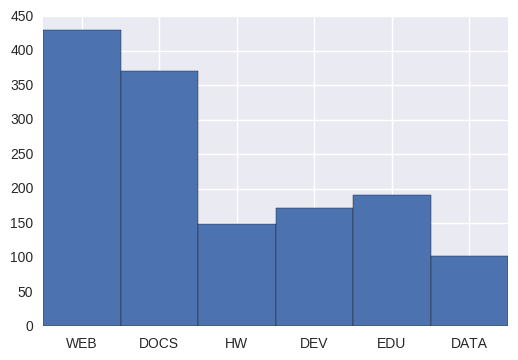
\includegraphics[max size={\textwidth}{\textheight}]{graphics/training_data_distribution.png}
	\caption{Training Data Distribution}
	\label{training_data_distribution}
\end{figure}

As one can see in the table \ref{data_sources}, we tried to use key words for automated searching that are as close to the words that were used to describe the different classes as possible.
Though, it's still possible that the collected training data is biased as we actively selected repositories by searching for them.
As an extension, an approach that could minimize this bias would be to randomly select repositories (e.g.~from the GHTorrent project) and label them manually.
For the beginning, however, we neither had the time nor the manpower to label a large amount of repositories manually.
Since the difficulty to collect data entries of a certain label differed, we ended up with unbalanced training data.
As the class label distribution affects some classifiers heavily, we trained the models on randomly undersampled training data.

\subsection{Data Analysis}\label{data-analysis}

To get a better idea of how the relationships between the data entries look like in a higher dimensional space, we used principal component
analysis (PCA) and t-distributed stochastic neighbor embedding (t-SNE) to reduce the complexity of the data to 2D while retaining the principal
components respectively the distances between the data points.
The figure \ref{t-sne-training-data} visualizes the distribution of the labeled data entries using t-SNE.

\begin{figure}
	\centering
		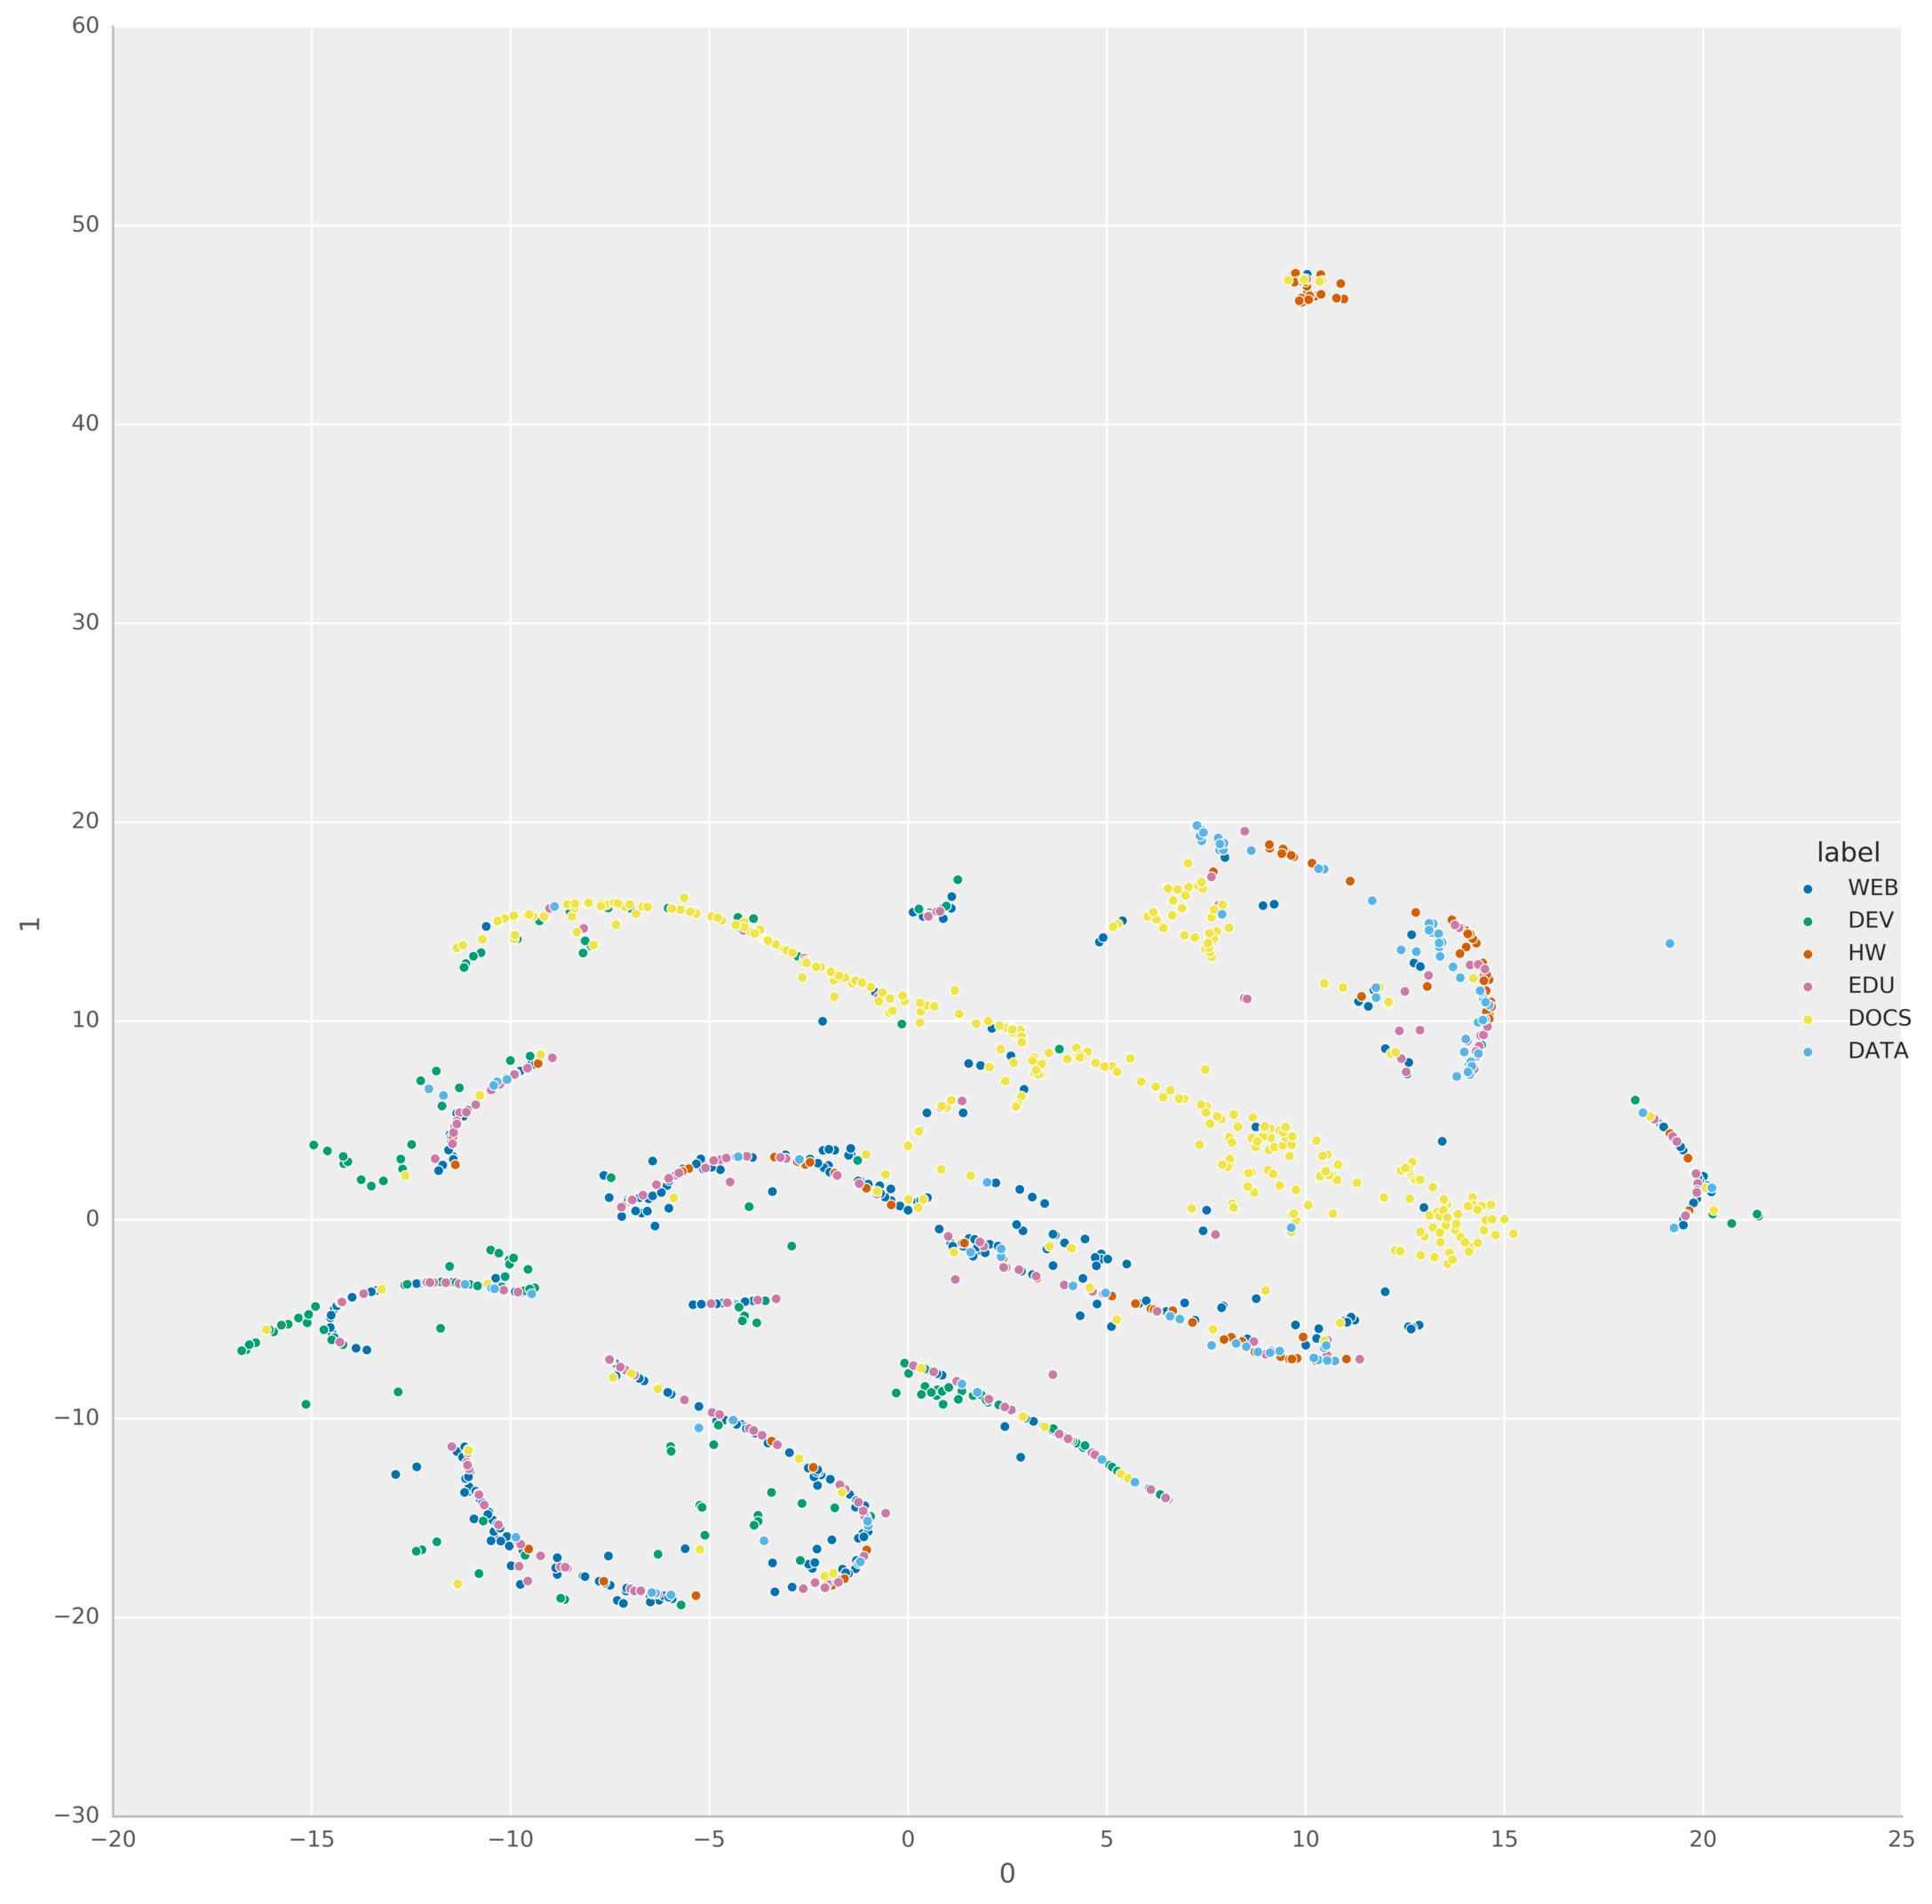
\includegraphics[max size={\textwidth}{\textheight}]{graphics/t-sne-training-data.png}
	\caption{Distribution of the labeled data entries using t-SNE}
	\label{t-sne-training-data}
\end{figure}

You can find the complete code to generate the figure in the t-SNE Visualization Notebook\footnote{https://github.com/WGierke/git\_better/blob/master/t-SNE\%20Visualization.ipynb}.
To explore the data interactively and in a three dimensional reduction you can use the Tensorflow Embedding Projector setup\footnote{https://github.com/WGierke/git\_better\#usage}.
One can notice that the ``DOCS'' repositories build a cluster while it seems to be more complicated to separate the other classes.

We also used t-SNE to visualize the similarity between our retrieved training data and the given validation data as you can see in figure \ref{t-sne-validation-data}.

\begin{figure}
	\centering
		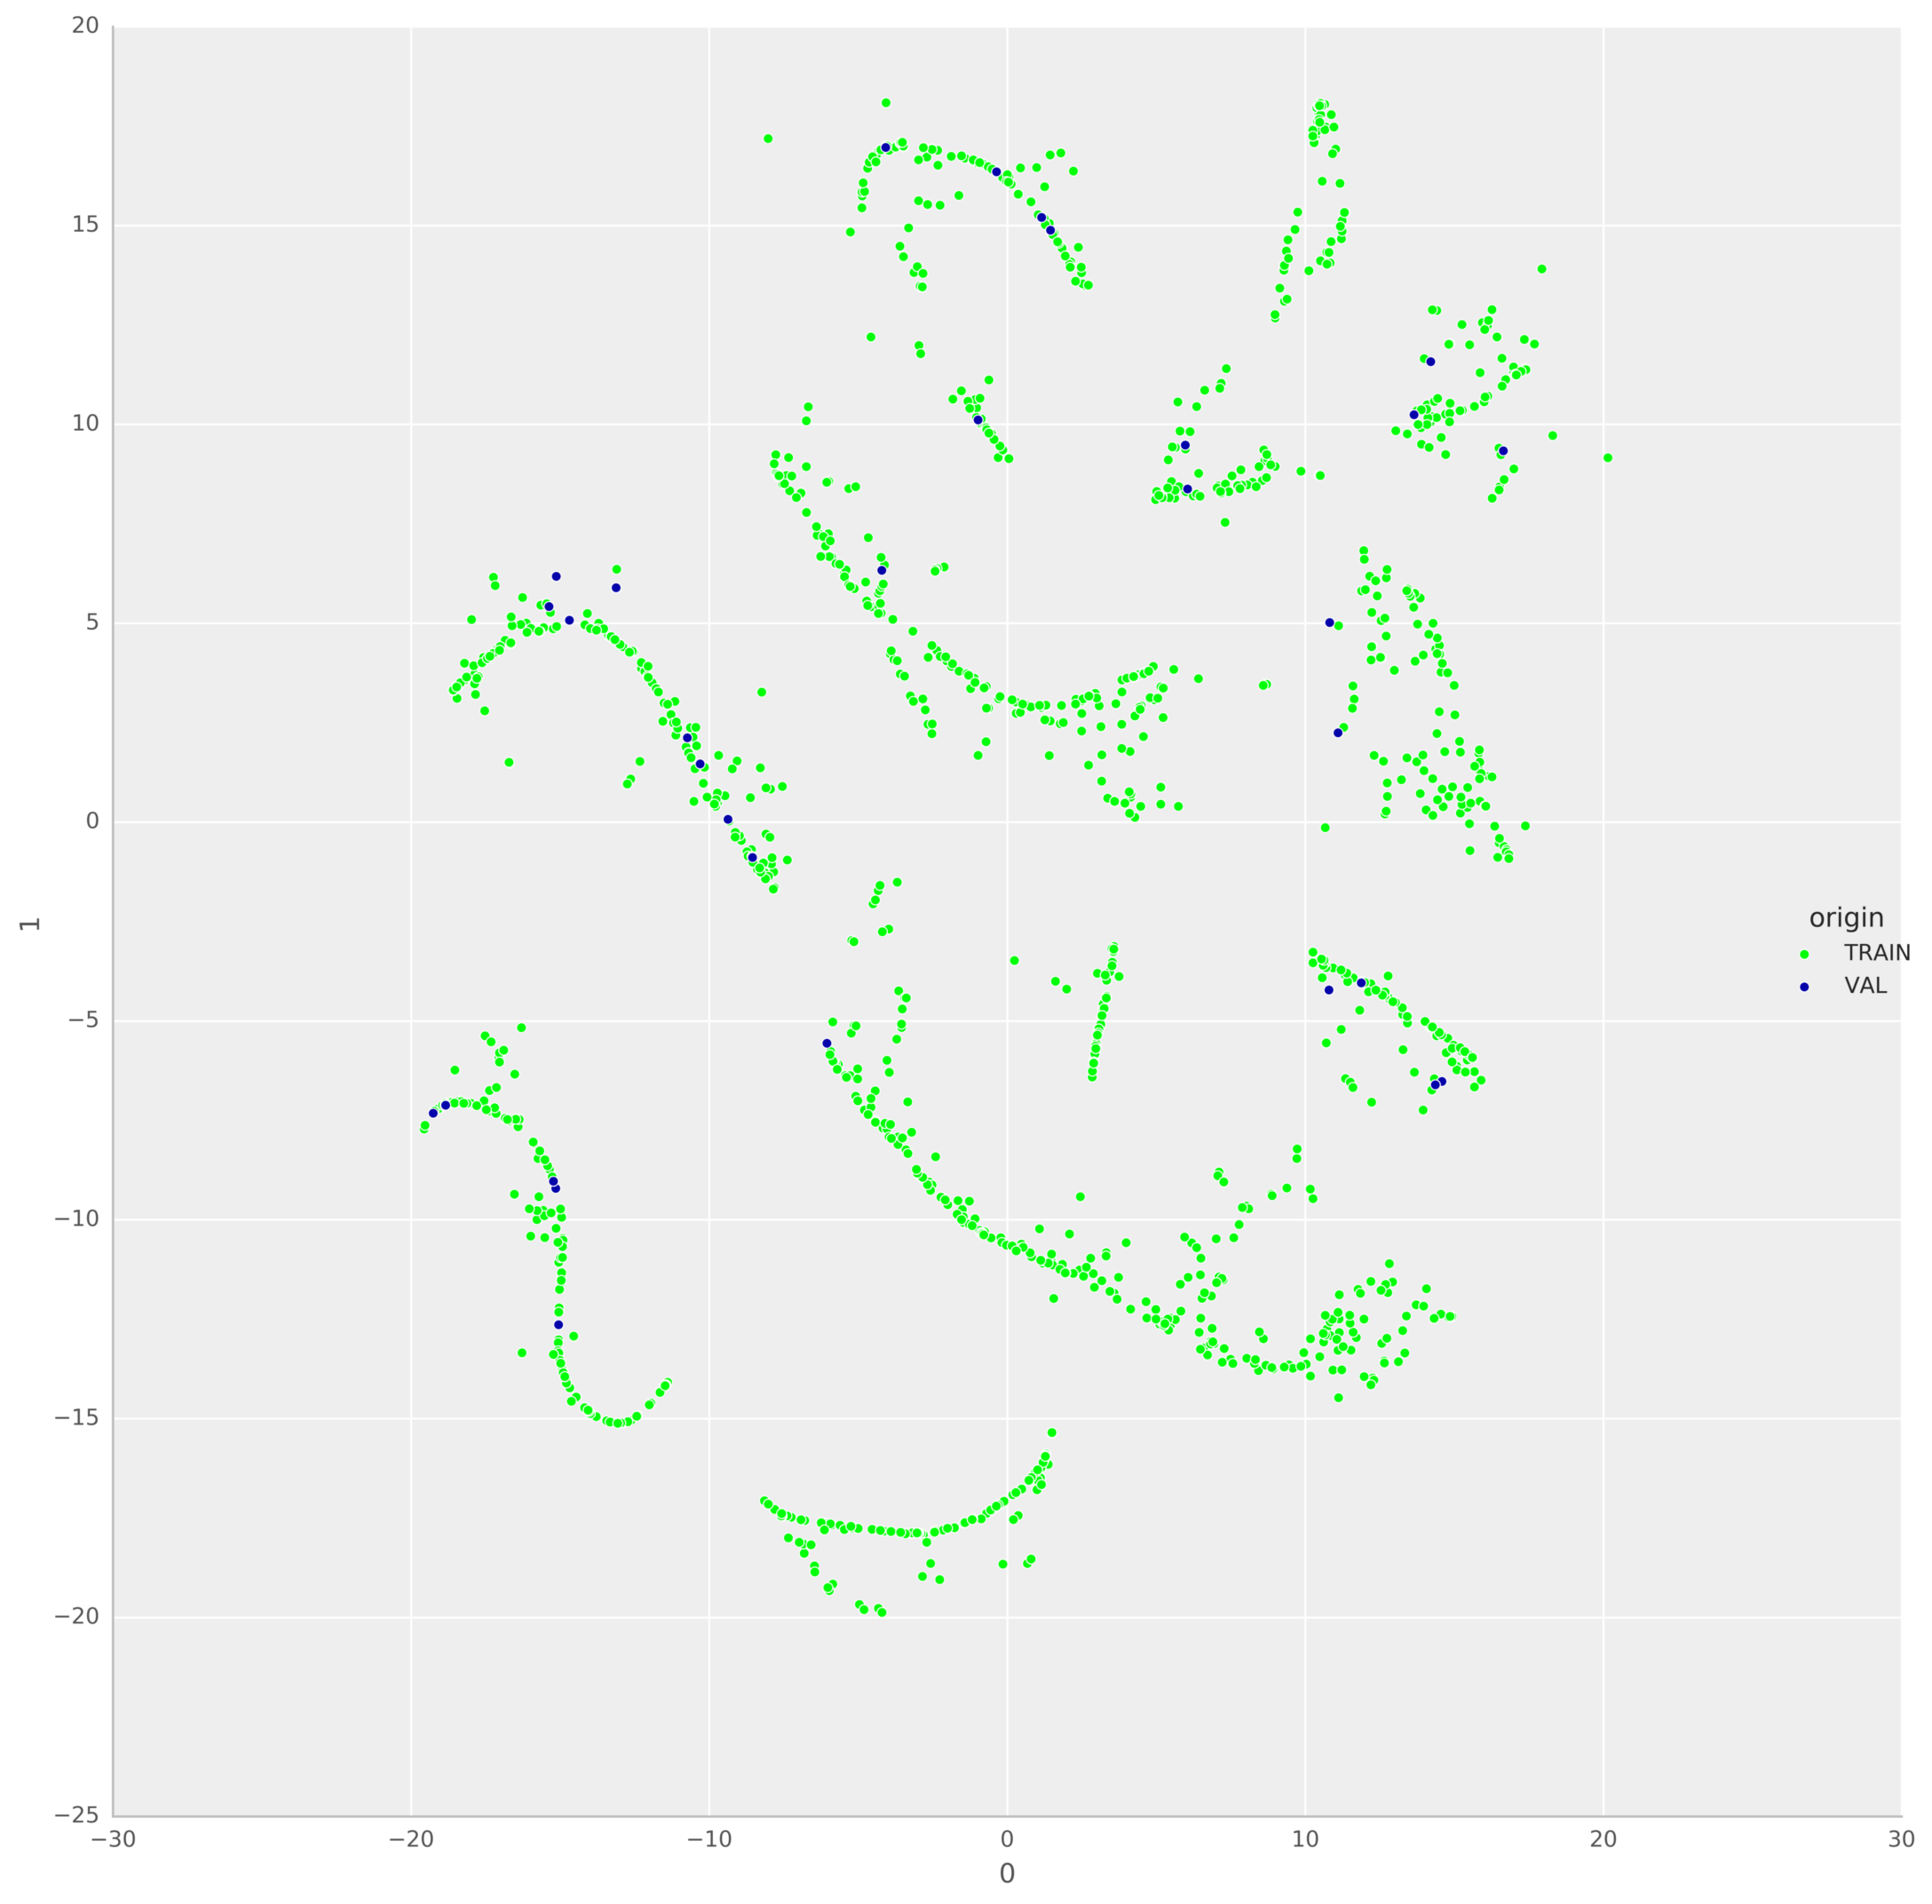
\includegraphics[max size={\textwidth}{\textheight}]{graphics/t-sne-validation-data.png}
	\caption{Distribution of the validation data entries using t-SNE}
	\label{t-sne-validation-data}
\end{figure}

Since the validation data does not form separate clusters or outliers, we could assume that testing the learned models on the validation data
is a good way to verify how well the models generalize.
On the other side, the validation data only contains roughly 30 data entries which is not enough to give reliable statements about the model performances.
Furthermore, the fact that the validation data seems to be selected manually implies that it's also biased.
Thus, perfect validation data would be a lot of randomly selected repositories that have been labeled manually.
The additional data sets\footnote{https://github.com/InformatiCup/InformatiCup2017/tree/master/additional\_data\_sets} from another team could allow us to validate our models better even if they are also biased.
As already mentioned, a perfect training and validation set would only contain repositories that have been sampled randomly and labeled manually.

\section{Prediction Model}\label{prediction-model}

When a model fits its training data too well and doesn't learn to generalize, it's considered to ``overfit''.
This can occur if the model is too complex so it learns the training data by heart instead of understanding how to solve the given problem in general.
To prevent this, we collected more training data than we already received by the challenge, we applied regularization to hinder the model becoming too complex and we used ensemble learning.\\
By collecting more data than already given we created a bigger problem domain that needs to be understood by the model.\\
Regularization adds a measure of the models complexity to the cost function that needs to be optimized.
Thus, the model does not only try to solve the given problem but it also tries to do that keeping itself as simple as possible.\\
Ensemble learning uses multiple trained models to calculate one final prediction.
These models are trained using distinct features so they're not related to each other.
The assumption is that when one model makes a mistake predicting a label, the other models don't make a mistake in this situation so the (correct predicted) label of the other models is returned.
To decide which model prediction is the correct one we used the Majority Rule algorithm.
One model was trained on the numerical features of a repository, one on the description, one on the content of the readme and one on the source code of each repository.\\
The following chapters will explain how we retrieved and cleaned the data for each model, how we selected relevant features and how we developed the prediction model.

\subsection{Training and Test Data
Set}\label{training-and-test-data-set}

To train and evaluate the classifiers, we used a train/test/validation split.\\
First, the collected training data was splitted in a train and a test split in a stratified manner.
This ensured that the distribution of class labels was balanced in both splits.\\
The classifiers were then trained on the train split and their accuracy was evaluated on the test split.
To calculate their final quality, we evaluated them on the validation data.

\subsection{Classification Using Numeric Metadata of
Repositories}\label{classification-using-numeric-metadata-of-repositories}

To develop classifiers based on numeric metadata of repositories, we used the features explained in table \ref{features}.

\begin{table}[]
\centering
\caption{My caption}
\label{features}
\begin{tabularx}{\linewidth}{|l|X|}
\hline
Feature Name           & Description                                                                        \\ \hline
watchers               & Number of users who watch the repo                                                 \\ \hline
mentionableUsers       & Number of mentionable users (collaborators, contributors, ...)                     \\ \hline
open\_pull\_requests   & Number of open pull requests                                                       \\ \hline
closed\_pull\_requests & Number of closed pull requests                                                     \\ \hline
merged\_pull\_requests & Number of merged pull requests                                                     \\ \hline
open\_issues           & Number of open issues                                                              \\ \hline
closed\_issues         & Number of closed issues                                                            \\ \hline
forks                  & Number of forks                                                                    \\ \hline
stargazers             & Number of users who "starred" the repo                                             \\ \hline
projects               & Number of projects (integrated project management tool)                            \\ \hline
size                   & Size of the source code in kilobyte                                                \\ \hline
isOwnerHomepage        & Is the name of the repo REPO\_OWNER.github.io or REPO\_OWNER.github.com?         \\ \hline
hasHomepage            & Does the website \newline{}REPO\_OWNER.github.io/REPO\_NAME exist?                           \\ \hline
hasLicense             & Does the repo have a license file?                                                 \\ \hline
hasTravisConfig        & Does the repo have a Travis configuration file?                                    \\ \hline
hasCircleConfig        & Does the repo have a CircleCI configuration file?                                  \\ \hline
hasCiConfig            & hasTravisConfig OR hasCircleConfig                                                 \\ \hline
commitsCount           & Number of commits                                                                  \\ \hline
branchesCount          & Number of branches                                                                 \\ \hline
tagsCount              & Number of tags                                                                     \\ \hline
releasesCount          & Number of releases                                                                 \\ \hline
LANGUAGE\_*            & How much code was written in the language in percent (e.g. LANGUAGE\_Python, ...)? \\ \hline
\end{tabularx}
\end{table}

Most of the features were available using the GitHub API.
We added the \emph{isOwnerHomepage} and \emph{hasHomepage} features to detect whether a repository serves its source code using GitHub pages.
This could allow us to identify WEB repositories easier.
We furthermore hoped that using \emph{hasCiConfig}, so whether a repo contains a configuration file for a Continuous Integration service, would improve the accuracy of detecting DEV repositories.

\subsubsection{Data Cleaning and
Preprocessing}\label{data-cleaning-and-preprocessing}

Using the GitHub REST API and the GitHub GraphQL API, we were able to receive all features without extensive cleaning or preprocessing of the data.

\subsubsection{Feature Selection}\label{feature-selection}

Feature Selection describes the process of dropping features that yield no or very little additional information in order to decrease overfitting and accelerate model fitting.
Especially the programming language features needed to be reduced using Feature Selection.\\
GitHub detects over 300 used programming languages\footnote{https://github.com/github/linguist/blob/master/lib/linguist/languages.yml} in repositories.
The problem is that a lot of them are used only in a few repositories such that there are a lot of features that only hold very little variance and information.
As an example, among the collected 1400 repositories there were 46 programming languages, like Pony or KiCad, that were only used in one repository at all.
To remove those, we dropped features with low standard deviation and a low overall sum.
As an example, we are already able to drop 135 language features if we require that the sum of a language feature over all 1400 training data entries is supposed to be bigger than 5.

\subsubsection{Feature Engineering}\label{feature-engineering}

In a next step, we derived further features from the features we already collected.
We used polynomial feature generation which takes the input variables and builds all possible polynomial combination of this features up to a given degree.
The idea of taking input features and applying a non-linear method on it to map the original values in another space is called ``kernel trick'' and is used by Support Vector Machines (SVM) to learn non-linear models as well.\\
As an example, suppose a dataset is given with the two features \textit{size} and \textit{watchers} as in table \ref{example-feature-engineering-basic}.

\begin{table}[]
\label{example-feature-engineering-basic}
\centering
\caption{Original features}
\begin{tabular}{|r|r|}
\hline
size & watchers \\ \hline
2    & 5        \\ \hline
10   & 8        \\ \hline
\end{tabular}
\end{table}

The transformed dataset using polynomial features with a degree up to 2 would look like table \ref{example-feature-engineering-transformed}.

\begin{table}[]
\label{example-feature-engineering-transformed}
\centering
\caption{Polynomially generated features (degree=2)}
\begin{tabular}{|r|r|r|r|r|}
\hline
size$^1$ & watchers$^1$ & size$^1\cdot$watchers$^1$ & size$^2$ & watchers$^2$ \\ \hline
2 & 5 & 10 & 4 & 25 \\ \hline
10 & 8 & 80 & 100 & 64 \\ \hline
\end{tabular}
\end{table}

As one can see, the number of generated features increases polynomially in the number of input features.
That's why the previous Feature Selection step was very important.

As alternative we could have used deep learning techniques but you need many training samples because of their higher learning complexity.
Our \textasciitilde{}1500 samples aren't enough for this.
Small feed-forward neural networks are applicable to our problem while deep neural networks are not.

\subsubsection{Numeric Metadata Prediction
Model}\label{numeric-metadata-prediction-model}

We tried the following classifiers: \ldots{}

{[}Better without language features{]}

{[}accuracy from single models{]}{[}accuracy from ensembled models{]}

\subsubsection{Validation of Prediction
Model}\label{validation-of-prediction-model}

{[}accuracy+confusion matrix{]}

\subsection{Classification Using Text Data (Description and
Readme)}\label{classification-using-text-data-description-and-readme}

Intuitively, one wouldn't use the numeric features like the number of branches etc. to decide what label fits the repository best.
Instead, one would use the description or the content of the readme to determine it.
For this reason we used term frequency--inverse document frequency (tf-idf) matrices to develop natural language processing (NLP) models that predict the label based on them.
Since there's a semantic difference between the description and the readme of a repository, we discarded the idea of concatenating the text features and training one model on it.
Instead, we trained two seperate models on the description respectively readme of the repositories.

\subsubsection{Data Cleaning and
Preprocessing}\label{data-cleaning-and-preprocessing-1}

To remove words like `the', `a', `and' etc. that occur very often and yield little meaning, we used the Natural Language Toolkit (NLTK) to drop English stopwords.
Since it's also not important whether the singular or the plural of words are used, we also used this toolkit to stem English words.

\subsubsection{Feature Generation from Existing
Data}\label{feature-generation-from-existing-data}

We used a count vectorizer which converts a text into a n-dimensional vector representing the vocabulary, where n is the number of unique words.
After this text-to-vector conversion we transformed the vector into a tf-idf vector which is a normalized representation of the original vector.

[Include positive and negative words]

\subsubsection{Feature Selection}\label{feature-selection-1}

{[}removal of rare/frequent words and stopwords{]}

\subsubsection{Prediction Model}\label{prediction-model-1}

Based on our tf-idf vector we can classify the different repositories using the n-dimensional vector as features and normal classification algorithms.

\subsubsection{Validation of Prediction
Model}\label{validation-of-prediction-model-1}

\begin{figure}
	\centering
		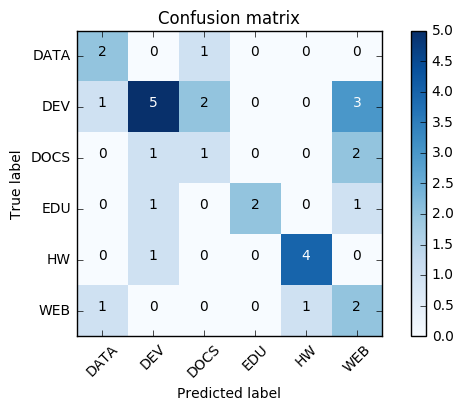
\includegraphics[max size={\textwidth}{\textheight}]{graphics/confusion-matrix-readme-classifier.png}
	\caption{Readme Classifier: 51.6\% Accuracy on Validation Data}
	\label{confusion-matrix-readme-classifier}
\end{figure}

\begin{figure}
	\centering
		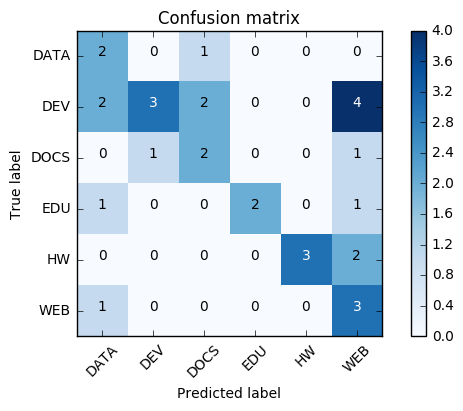
\includegraphics[max size={\textwidth}{\textheight}]{graphics/confusion-matrix-description-classifier.png}
	\caption{Description Classifier: 48.4\% Accuracy on Validation Data}
	\label{confusion-matrix-description-classifier}
\end{figure}

{[}Include images with additional validation data{]}

\subsection{Classification Using Source
Code}\label{classification-using-source-code}

We tested different approaches to use the source code and connected data of a repository to classify it.
For this task we used only data included in the git repository, no github specific data like projects, the wiki pages\ldots{} Data from the repositories are including source code files with comments and git workflow specific data (branches, commits\ldots{}).
We used in this chapter mainly the source code, file names and commit messages.

\subsubsection{Data Cleaning and
Preprocessing}\label{data-cleaning-and-preprocessing-2}

We cloned each repository locally to retrieve the data we need.
After this step we were able to merge all non-binary source code files, all filenames and all git commit messages into three different files.
We didn't filter based on languages and all UTF-8 files are included.
This could be an additional preprocessing step to improve and simplify the stemming and classification.

\subsubsection{Feature Generation from Existing
Data}\label{feature-generation-from-existing-data-1}

We were able to use the same feature generation approach based on the count vectorizer and tf-idf vector as used in the text data classification.
Ugurel et al.\footnote{"What's the Code? Automatic Classification of Source Code Archives", KDD, 2002} showed a similar approach successfully.

[Include positive and negative words]

\subsubsection{Feature Selection}\label{feature-selection-2}

{[}removal of rare/frequent words and stopwords{]}

\subsubsection{Prediction Model}\label{prediction-model-2}

{[}Same as text data{]}

\subsubsection{Validation of Prediction
Model}\label{validation-of-prediction-model-2}

{[}accuracy+confusion matrix{]}

\subsection{Overall Prediction
Model}\label{overall-prediction-model}

\begin{itemize}
\tightlist
\item
  {[}Describe our ensembled model{]}
\item
  {[}Document three repositories which work well{]}
\end{itemize}

\section{Implemented Application}\label{implemented-application}
\subsection{Tooling Choices}\label{tooling-choices}
\subsection{Functionality}\label{functionality}

Our implemented application takes a file containing GitHub repository URLs, classifies them using an ensemble model that's trained on passed training data and saves the URLs and their computed labels on the disk.
If no training data is given, the input data will be classified using our pre-trained model.
It's possible to pass the input data, which is supposed to have the format of the challenge example\footnote{https://github.com/InformatiCup/InformatiCup2017/blob/master/example-input}, using the \texttt{-i} argument.
Optional training data can be passed using the \texttt{-t} argument.\\
As an example, to classify the example data given by the challenge using the training data given by the challenge one would run:

\begin{lstlisting}[language=bash]
  $ python app/main.py -i data/example-input.txt
                       -t data/training_data_small.csv
\end{lstlisting}

The saved output file \texttt{predictions.txt} will have the format of the challenge example\footnote{https://github.com/InformatiCup/InformatiCup2017/blob/master/example-output}.\\
For setup instructions please refer to the README.md file.

\section{Validation}\label{validation}

\begin{itemize}
\tightlist
\item
  {[}boolean(!) matrix on validation data{]}
\item
  {[}compute recall and precision{]}
\item
  {[}discuss quality of results and whether higher yield or higher
  precision is more important{]}
\item
  {[}(elaborate on the additional dataset given by another team?){]}
\end{itemize}

\section{Extensions}\label{extensions}

To bring our research work to production, we built a service\footnote{https://git-better.herokuapp.com/} that classifies your public GitHub repositories using models that were trained on our training data.
The server uses GitHub OAuth to authenticate GitHub users and uses their OAuth tokens to request their public repositories and their necessary features.
We're planning to improve the design with visualizations of the repository distribution using D3.\\
Another extension would be to recommend trending GitHub projects\footnote{https://github.com/trending} based on the public repositories of the user.\\
Since there is no official GitHub API for the trending repositories, we would crawl all websites that are available at \\
https://github.com/trending/\textit{language}?since=\textit{since} once a day, where \textit{language} is a supported programming language like Python or Ruby, and \textit{since} is one of `daily', `weekly' or `monthly'.
We would then recommend repositories to the user based on their classified labels, on the preferred language of the user, on the text or even code similarity between the trending projects and those of the user.
To implement the latter one, we could use tf-idf matrices like we already used for the text classifiers.

\begin{itemize}
\tightlist
\item
  {[}maybe add pictures as fall-back{]}
\end{itemize}

\newpage
\appendix
\section{\\Evaluation of file name classifier} \label{App:AppendixA}
% the \\ insures the section title is centered below the phrase: AppendixA

\begin{table}[h]
\centering
\caption{Classifier on file names - DATA category}
\label{file-names-data}
\begin{tabular}{|l|l|l|l|l|}
 \hline
   & \multicolumn{2}{l}{Positive words} & \multicolumn{2}{l}
{Negative words} \\ \hline
1 & 3.2251  &              json  &  -1.5670  &           packag \\  \hline
2 & 1.1139  &           makefil  &  -1.5648  &             test \\  \hline
3 & 0.9449  &                sh  &  -1.5623  &             main \\  \hline
4 & 0.6635  &               xml  &  -1.4399  &           config \\  \hline
5 & 0.6452  &                py  &  -1.1262  &              png \\  \hline
6 & 0.4514  &             readm  &  -1.0827  &              yml \\  \hline
7 & 0.3790  &            licens  &  -0.9016  &        contribut \\  \hline
8 & 0.3784  &             index  &  -0.7405  &              jpg \\  \hline
9 & 0.3127  &               txt  &  -0.4513  &              css \\  \hline
10 & 0.1726  &          gitignor  &  -0.2326  &            travi \\  \hline
11 & 0.0919  &               pdf  &  -0.2206  &             util \\  \hline
12 & 0.0861  &                md  &  -0.1236  &             html \\  \hline
13& &  &  -0.0684  &              svg \\  \hline
14& &  &  -0.0304  &               js \\  \hline
\end{tabular}
\end{table}
\begin{table}[h]
\centering
\caption{Classifier on file names - DEV category}
\label{file-names-dev}
\begin{tabular}{|l|l|l|l|l|}
 \hline
   & \multicolumn{2}{l}{Positive words} & \multicolumn{2}{l}
{Negative words} \\ \hline
1 & 3.4637  &              util  &  -1.9203  &              pdf \\  \hline
2 & 2.3105  &            packag  &  -1.0563  &            travi \\  \hline
3 & 1.8472  &               yml  &  -0.9946  &              css \\  \hline
4 & 1.7875  &              test  &  -0.5838  &            readm \\  \hline
5 & 1.4706  &                sh  &  -0.5619  &               md \\  \hline
6 & 1.4247  &                js  &  -0.3192  &         gitignor \\  \hline
7 & 1.3238  &              html & & \\  \hline
8 & 1.2926  &           makefil & & \\  \hline
9 & 0.9907  &            config & & \\  \hline
10 & 0.9156  &              main & & \\  \hline
11 & 0.7826  &               png & & \\  \hline
12 & 0.7679  &            licens & & \\  \hline
13 & 0.7235  &             index & & \\  \hline
14 & 0.7082  &               xml & & \\  \hline
15 & 0.5805  &               txt & & \\  \hline
16 & 0.4977  &                py & & \\  \hline
17 & 0.3078  &         contribut & & \\  \hline
18 & 0.2526  &              json & & \\  \hline
19 & 0.1224  &               jpg & & \\  \hline
20 & 0.0541  &               svg & & \\  \hline
\end{tabular}
\end{table}
\begin{table}[h]
\centering
\caption{Classifier on file names - DOCS category}
\label{file-names-docs}
\begin{tabular}{|l|l|l|l|l|}
 \hline
   & \multicolumn{2}{l}{Positive words} & \multicolumn{2}{l}
{Negative words} \\ \hline
1 & 4.5622  &         contribut  &  -1.0314  &           config \\  \hline
2 & 2.8728  &             travi  &  -1.0044  &             html \\  \hline
3 & 2.0420  &               yml  &  -0.7121  &              xml \\  \hline
4 & 1.7639  &            licens  &  -0.6340  &             json \\  \hline
5 & 1.7214  &                md  &  -0.5722  &          makefil \\  \hline
6 & 1.2027  &            packag  &  -0.5702  &             main \\  \hline
7 & 1.1108  &               svg  &  -0.5697  &             test \\  \hline
8 & 0.6831  &               png  &  -0.5455  &               sh \\  \hline
9 & 0.6714  &             index  &  -0.4359  &               py \\  \hline
10 & 0.3497  &             readm  &  -0.4040  &              txt \\  \hline
11 & 0.2890  &               css  &  -0.3430  &               js \\  \hline
12 & 0.2780  &               jpg  &  -0.2187  &              pdf \\  \hline
13& &  &  -0.1440  &             util \\  \hline
14& &  &  -0.0722  &         gitignor \\  \hline
\end{tabular}
\end{table}
\begin{table}[h]
\centering
\caption{Classifier on file names - EDU category}
\label{file-names-edu}
\begin{tabular}{|l|l|l|l|l|}
 \hline
   & \multicolumn{2}{l}{Positive words} & \multicolumn{2}{l}
{Negative words} \\ \hline
1 & 1.7966  &               pdf  &  -1.9717  &        contribut \\  \hline
2 & 1.5195  &              html  &  -1.2080  &              yml \\  \hline
3 & 1.3308  &               jpg  &  -1.1482  &             util \\  \hline
4 & 1.0053  &               svg  &  -0.8443  &             json \\  \hline
5 & 0.9685  &               png  &  -0.2571  &           packag \\  \hline
6 & 0.8496  &          gitignor & & \\  \hline
7 & 0.6726  &                py & & \\  \hline
8 & 0.6248  &           makefil & & \\  \hline
9 & 0.5158  &            licens & & \\  \hline
10 & 0.4517  &               css & & \\  \hline
11 & 0.4501  &               txt & & \\  \hline
12 & 0.4491  &               xml & & \\  \hline
13 & 0.4232  &                sh & & \\  \hline
14 & 0.3983  &                js & & \\  \hline
15 & 0.3342  &              main & & \\  \hline
16 & 0.3019  &              test & & \\  \hline
17 & 0.2778  &             readm & & \\  \hline
18 & 0.1407  &                md & & \\  \hline
19 & 0.1085  &             travi & & \\  \hline
20 & 0.1042  &            config & & \\  \hline
\end{tabular}
\end{table}
\begin{table}[h]
\centering
\caption{Classifier on file names - HW category}
\label{file-names-hw}
\begin{tabular}{|l|l|l|l|l|}
 \hline
   & \multicolumn{2}{l}{Positive words} & \multicolumn{2}{l}
{Negative words} \\ \hline
1 & 2.0428  &               css  &  -1.5755  &        contribut \\  \hline
2 & 1.7615  &              main  &  -1.3501  &           licens \\  \hline
3 & 1.5388  &            config  &  -1.0360  &              yml \\  \hline
4 & 1.2715  &          gitignor  &  -0.8501  &            travi \\  \hline
5 & 0.9140  &               txt  &  -0.8123  &              svg \\  \hline
6 & 0.7449  &             readm  &  -0.8035  &             util \\  \hline
7 & 0.5342  &                py  &  -0.5982  &           packag \\  \hline
8 & 0.5257  &              test  &  -0.4826  &             json \\  \hline
9 & 0.4687  &               xml  &  -0.3102  &          makefil \\  \hline
10 & 0.4144  &             index  &  -0.2012  &               sh \\  \hline
11 & 0.3984  &               pdf  &  -0.1943  &             html \\  \hline
12 & 0.3699  &                js  &  -0.1773  &              png \\  \hline
13 & 0.3128  &                md & & \\  \hline
14 & 0.2245  &               jpg & & \\  \hline
\end{tabular}
\end{table}
\begin{table}[h]
\centering
\caption{Classifier on file names - WEB category}
\label{file-names-web}
\begin{tabular}{|l|l|l|l|l|}
 \hline
   & \multicolumn{2}{l}{Positive words} & \multicolumn{2}{l}
{Negative words} \\ \hline
1& &  &  -2.4446  &               md \\  \hline
2& &  &  -2.0628  &            readm \\  \hline
3& &  &  -1.9461  &               js \\  \hline
4& &  &  -1.9392  &              txt \\  \hline
5& &  &  -1.9117  &             html \\  \hline
6& &  &  -1.9110  &              png \\  \hline
7& &  &  -1.8890  &             json \\  \hline
8& &  &  -1.8842  &               py \\  \hline
9& &  &  -1.8702  &              xml \\  \hline
10& &  &  -1.8512  &              pdf \\  \hline
11& &  &  -1.8435  &         gitignor \\  \hline
12& &  &  -1.7930  &            travi \\  \hline
13& &  &  -1.7274  &             test \\  \hline
14& &  &  -1.7246  &           config \\  \hline
15& &  &  -1.7224  &              jpg \\  \hline
16& &  &  -1.7115  &             main \\  \hline
17& &  &  -1.7010  &              css \\  \hline
18& &  &  -1.6888  &          makefil \\  \hline
19& &  &  -1.6295  &           licens \\  \hline
20& &  &  -1.6165  &            index \\  \hline
\end{tabular}
\end{table}



\newpage
\section{\\Title of Appendix B} \label{App:AppendixB}
% the \\ insures the section title is centered below the phrase: Appendix B

Text of Appendix B is Here


\end{document}
